\chapter{The Automated Executions Plug-in}
This chapter describes the Automated Execution plug-in that is responsible for handling
the setup, control flow and display of an automated execution run.
Although the plug-in is structured according to the model-view-controller pattern this
is not the structure that this chapter will to describe it. Instead this chapter will
follow the structure already used in the previous chapters. Which means the chapter will
consist of four parts:
\begin{enumerate}
 \item The setup of an automated execution run with a description of the wizard.
 \item The input to the automated execution. This section will describe the newly created interface.
 \item The control flow of the automation with the Automation Job and the Automation Wizard.
 \item The output of the automation run. In this section the new view and the results structure will
be described.
\end{enumerate}


\section{Automation Setup - The Wizard}
\label{section:AutoWizard}
\index{Wizard}
As described in Section \ref{section:AutoConceptsSetup} an Eclipse wizard will be used to set up the 
automated run. For easy access the button for opening the wizard (

\includegraphics[scale= 0.7]{kiemAutomated.png})
is located on the tool bars of both the Execution Manager and the Automated Execution view.

The Automation Wizard consists of two pages:
\begin{enumerate}
 \item The File Selection Page for selecting all files that should be involved in the automated run.
 \item The Property Setting Page for defining custom properties that the components should receive prior to
each iteration.
\end{enumerate}


\subsection{File Selection Page}
\label{section:FileSelectionPage}
\begin{figure}
  \centering
  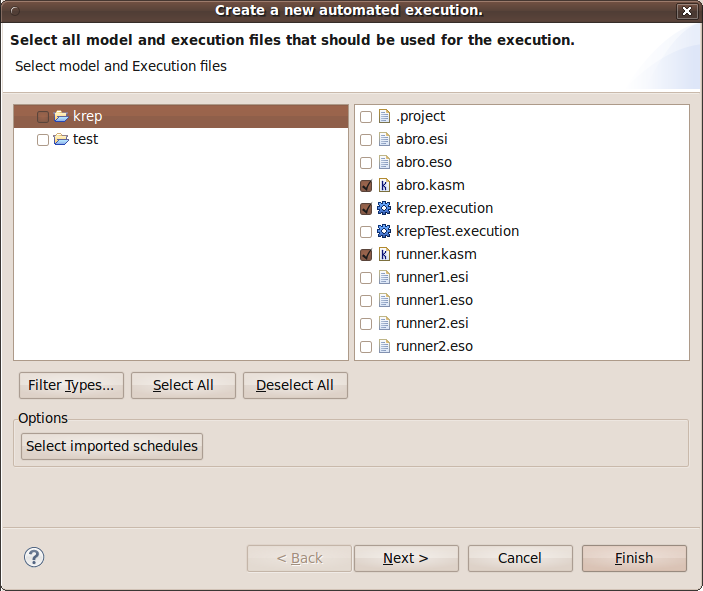
\includegraphics[scale=.4]{FileSelectionPage.png}
  \caption[The Wizard Page for selecting the input files for an automated run.]%
  {The Wizard Page for selecting the input files for an automated run.\protect}
  \label{fig:FileSelectionPage}
\end{figure}
The File Selection Page shown in Figure \ref{fig:FileSelectionPage} is used to select the model 
files and execution files that should be used for the automated run.

Since Eclipse already provides a variety of pre-made wizard pages it can be avoided to write a page for a
complex task like this from scratch. The wizard that can be modified to fit the needs of the task at hand
is the standard Eclipse Resource Import Wizard. It is normally used to select a number of files and folders
for import into the workspace. It provides a structured view where entire folders can be selected, files
can be filtered by their type and additional space is available for other buttons. In this project the files
will be 'imported' into the automated execution. This is similar enough to make it possible to use the wizard
with a few modifications and extensions.

As it should be as easy as possible to set up a run for the user it would be desirable that he doesn't need
to select all the files each time the wizard is opened. For this reason the selection will be saved into
the Eclipse preference store every time the wizard is closed. The next time the wizard is opened the selection
only has to be retrieved from the preference store and passed to the Resource Import Wizard super class.

The \ac{KIEMConfig} allows for execution files to be linked into the workspace through an extension
point. This is a useful feature for adding factory defaults and as such \ac{KIEMAuto} naturally wants to
be able to use these execution files as well. However since they these files are not in the workspace they
can't be selected through the main area of the wizard page. In order to select these files anyway a simple
list selection dialog can be accessed through the button at the bottom of the page. The dialog displays all
schedules imported through the extension point and allows the user to select any number of them.

The hard part is how to figure out if the user has selected valid files for an automated run. Recognizing selected
execution files can simply be done by looking at the file extension.
However determining whether the user selected valid model files that will work with the selected execution
files is somewhat difficult. One possibility would be to use the priority system in the \ac{KIEMConfig} in
order to determine the validity of the combinations. However this would assume that all selected execution files
are known to the plug-in and that the user set priorities for each of them. At this point it is simply assumed
that all selected files that have an extension other than 'execution' are model files. Precautions to avoid
running invalid combinations of model files and execution files are described in Section \ref{section:AutoInput}.

The dialog will only allow the user to proceed if at least one execution file or imported schedule and one
model file is selected. Otherwise an error marker will be displayed in the page header.

\subsection{Property Setting Page}
\label{section:PropertySettingPage}
\begin{figure}
  \centering
  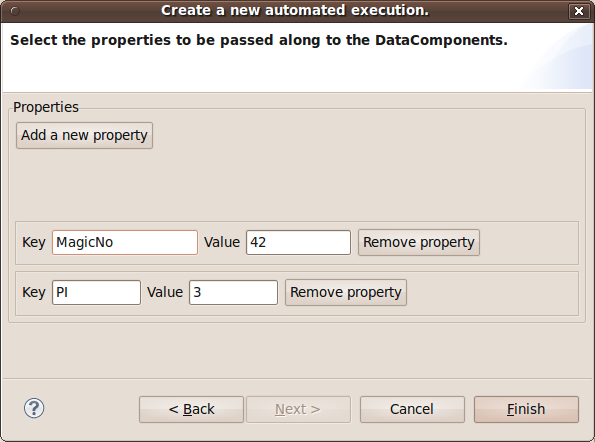
\includegraphics[scale=.4]{PropertySettingPage.png}
  \caption[The Wizard Page for setting up user defined properties.]%
  {The Wizard Page for setting up user defined properties.\protect}
  \label{fig:PropertySettingPage}
\end{figure}
The second wizard page shown in Figure \ref{fig:PropertySettingPage} allows the user to enter some custom
properties for the automated run. Unlike the first page this one doesn't extend a particular wizard page but
rather the generic wizard page that only supplies the header and the button bar at the bottom of the page.

The user can add an arbitrary number of panels for adding new (key, value) pairs through the button at the
top of the page. These values will be added to the list that is passed to all DataComponents before each iteration
and the values can be retrieved by looking for the key.

Since these properties are completely optional there are requirements for finishing this page. Which means that due
to the wizard nature of the dialog the user doesn't even have to look at that page at all but can finish directly
from the file selection page.

As with the file selection page the user input will also be stored as soon as the wizard closes and the properties
restored on the next opening of the wizard. The upside of which is that the user saves considerable work by only
having to enter the properties once. However the downside is that the user might not realize that the properties are
still set if he finishes the wizard directly from the first page. The only way to avoid this situation would be to
force the user to look at the second page. This is however very undesirable since the second page is likely to be used
only by advanced users anyway and the average user wouldn't want to see it.

\subsection{Information Processing}
\label{section:InformationProcessing}
After the user is finished with the wizard all information has to be collected in order to set up the automated run.
This involves the following steps:
\begin{enumerate}
 \item Gather the model files selected on the file selection page.
 \item Get the paths for the execution files. This might involve retrieving the paths from the schedules imported through
the extension point if the user selected any of those.
 \item Get the list of (key, value) pairs that should be added to the automated run from the second wizard page.
 \item Invoke the Automation Manager described in Section \ref{section:AutomatedRun} with the gathered parameters.
\end{enumerate}


\section{Automation Input}
\label{section:AutoInput}
In order to provide the DataComponents with input prior to each part of the automated run new interfaces
had to be created in order to interact with the components. 

\subsection{Automated Component}
\label{section:AutomatedComponent}
\index{Automated Component}
An automated component is any DataComponent (see Section \ref{section:IntroDataComponent}) that wants to interact with
the automated execution plug-in. An automated component has to provide the following methods:

\begin{description}
 \item \textbf{String[] getSupportedExtensions()} :

This method is used in order to avoid the automated run encountering errors while trying to
simulate invalid combinations of model files and execution files. As soon as any execution file
is loaded the method will be called on each of the implementing classes. The classes should answer
with a list of file extensions of the model files that they can simulate. Model files that no
component in the currently active execution file can simulate will be skipped.

 \item \textbf{void setParameters(List<KiemProperty> properties) throws KiemInitializationException} : 

This method enables components to receive information prior to each execution
run. The list is implemented as an array of key, value pairs stored inside
KiemProperty objects.
At the every least the list contains the location of the model file and the
index of the currently running iteration.
This allows components to load additional files that are always in the
same path as the execution file and determine which of those to load
based on the iteration index.
The custom properties that the user defined through the wizard for example are
also added here.
If the component encounters an error during at this point because for example a model file
could not be loaded it should respond by throwing the declared Exception.

 \item \textbf{int wantsMoreSteps()} : 

This method is called before the Automation Manager performs the first step.
All components will be asked how many steps they are likely to need for their
execution run. The maximum of these values will be taken and the execution
will perform the requested number of steps. After that the components
will be asked again and so on. The process stops when all components
answer with zero.

 \item \textbf{int wantsMoreRuns()} : 

This method works analog to the wantsMoreSteps() method in the context
of entire execution runs. It is used to determine how many iterations
should be performed with the given combination of execution file and model
file.
\end{description}

\subsection{Automated Producer}
\label{section:AutomatedProducer}
This interface extends the AutomatedComponent interface.
In addition to the inherited methods it provided one additional method.

\begin{description}
 \item \textbf{List<KiemProperty> produceInformation()} : 

This method is called after an iteration has finished and asks the components
if they want to publish any information about the results of their execution.
This information is gathered by the plug-in and the accumulated results
are either passed to the calling plug-in or displayed in the
specially designed view (see Section \ref{section:AutoView}).

The component is free to publish any amount of information using any of the 
different KiemProperty types. However the number and order of the properties
in the list has to stay the same through all iterations with one execution file.
This restriction is necessary in order to be able to build one large table
rather than many small ones.
\end{description}


\section{The Automated Run}
\label{section:AutomatedRun}
The Automation Manager is the key part of the automated execution. It manages the entire control flow
through the automated execution and its public methods are part of the plug-ins \ac{API}. The reason
for this is that the automated run can be initiated without the use of the wizard by any other
plug-in.

The next sections will give a detailed description of the control flow during the automated execution.
The \ac{API} methods to initiate a new automated execution are located inside the Automation Manager. However
since those methods immediately create a new Automation Job and schedule it right away the first section will
explain the Automation Job. 

Section \ref{section:AutomationManager} will then proceed to describe the entire control flow that is managed by the Automation Manager.

In Section \ref{section:CancelManager} the Cancel Manager will be described which is
responsible for triggering a premature termination of the entire automated execution or parts
of it.

The last section will describe the modifications to the ErrorHandler in order to ensure a smooth
run of the automation.

\subsection{Automation Job}
\label{section:AutomationJob}
\index{Automation Job}
The Automation Job is used to run the automated execution in. As a WorkbenchJob it can execute parallel
to the normal operation of the \ac{GUI} without blocking it. It also comes with a progress monitor that
is updated by the Automation Manager through the course of the automated execution. Since an automated run
can take a very long time the user can also tell the job to run in the background while still being able
to get feedback about it through Eclipse's progress view.

Upon creation the Automation Job takes all the parameters necessary for the automated execution. After that
it opens Execution Manager view in order to load all necessary plug-ins before the actual run starts. 
The job then creates a new thread and initiates the automated execution inside the Automation Manager.
At the end it tells the calling thread that it's returning asynchronously in order not to block any callers.

The dialog showing the progress monitor is not only used to get feedback about the progress of the task
it can also be used to cancel the execution prematurely for example if the user realizes that he selected
the wrong files.

\subsection{Automation Manager}
\label{section:AutomationManager}
\index{Automation Manager}
The Automation Manager is responsible for handling the entire control flow during the automated execution.
It takes the execution files, model files and other properties as arguments and organizes the entire
run based on the available information. During the run the Automation Manager also collects the information
that will be displayed as results by the view.

\begin{enumerate}
 \item \label{item:initiateProgressMonitor} The Automation Manager starts by initializing the 
progress monitor that displays the progress of the automated execution. 
The displayed message of the monitor is set up and the total length of the execution is 
calculated in order for the progress bar to be displayed.

Since a priori only the number of execution files and model files is known these are the only
variables that can be used. If more than one execution file and one model file are used the 
progress monitor will display a progress bar that advances with each completed model file. 
However this method would be meaningless if only one execution file and one model file
are used. In this case the progress bar will just show that progress is occurring at all.

 \item \label{item:saveOpenedFile} In this step the Automation Manager stores the path
of the execution file that is currently opened inside the Execution Manager. The reason for this
is that the user might want to continue working on that file after the automated execution
has finished. If the file wasn't stored he would be left with the last execution file
that the automated run simulates. The file is restored in Step \ref{item:restoreFile}.

 \item \label{item:initiateCancelManager} The next step is to initiate the Cancel Manager
described in Section \ref{section:CancelManager}. This also involves registering as listener on the 
modified ErrorHandler (see Section \ref{section:ErrorHandler}) to prevent any Exception
from interfering with the automated run.

 \item \label{item:checkExecutionFile} Since all parameters for the automated execution
have been set up now the Automation Manager can start working on the first execution file. The first
thing to do here is to open the execution file inside the Execution Manager. If this fails the automation
writes an entry into the error log and proceeds to the next execution file. Otherwise it proceeds to the
next step. If all execution files have finished the automation will skip to Step \ref{item:automationDone}.

 \item \label{item:setupExecutionFile} The next step is to initiate all variables that are needed
for the currently active execution file. The manager first asks the view to create a new table to
display the results that the execution will produce. After that all components will be asked
for the list of model file extensions that they support (see Section \ref{section:AutomatedComponent}).

 \item \label{item:checkModelFile} With the information about the supported model file extensions
gathered in the previous step the automation can start to examine the first model file. If any component
in the current execution file supports the given model file the automation proceeds to the next step.
Otherwise it skips to the next model file. If all model files on the current execution file
have finished it will proceed to Step \ref{item:checkExecutionFile} with the next execution file.

 \item \label{item:notifyObservers} The first thing that happens when the Automated Manager decides
that a model file should be simulated is that all Automated Components will be notified with the
list of parameters. 

This method iterates over all components and provides them with the list
of user defined properties that were passed to the automated execution. The list also includes
the path of the current model file and the index of the current iteration. Some components
may choose to write information back into the list in order to communicate with other
components. Therefore the list will be passed to all components twice if the size changed
between after the first notification.

 \item \label{item:askForRuns} Since the components now have all the necessary information for
the first iteration they might already be able to approximate how many iterations they want to
execute. Therefore all components will be asked through the methods provided in the interface
and the maximum value used.

At this point all components may decide that they don't need any runs
at all. The automation will then add a new result to the panel displaying that fact. After that
the automation will continue on Step \ref{item:checkModelFile} with the next model file.

If any component answers with a non-zero value the automation will move to the next step and
perform at least that many iterations, baring user cancellation of course.

 \item \label{item:checkIteration} Since set up of the model file has now finished the 
automation now checks if an iteration should be executed. It first checks whether the
number of remaining iterations has reached zero in which case no component requested
another run. It then checks whether the current model file was skipped through the 
Cancel Manager (see Section \ref{section:CancelManager}). If both checks turn out to 
be negative it proceeds to the next step after decrementing the amount of remaining
iterations. If one of the checks hold true it continues on Step \ref{item:checkModelFile}
with the next model file.

 \item \label{item:setupIteration} In this step the Automation Manager sets up all 
parameters that are needed for the current iteration.

It starts by updating the text in the progress monitor in order to reflect the
current status of the automation. The displayed text shows the current model file
and execution file, the iteration index and how many iterations are to be expected
based on the value retrieved from the components.

After that the manager adds a new row to the resulting table inside the view (see Section
\ref{section:AutoView}). This has to be done at this stage in order to show the 
status of the currently executing iteration before it has finished.

Before the execution can proceed the components first have to be passed the list
of parameters including the current iteration index. This process is performed by
the same method as described in Step \ref{item:notifyObservers}.

After all the preparations have been completed the automation proceeds to the next
step.
 
 \item \label{item:initExecution} The next step is to access the Execution Manager
itself in order to initialize the execution. The Execution Manager will set up all
DataComponents and create the thread in which the execution is run.

If an error occurred at this stage the automation will skip to Step \ref{item:IterationWrapup}.
An error can be caused by any of the DataComponents during their initialization phase or
by the Execution Manager itself if the execution file can be loaded but not executed.

If the initialization was successful the Automation Manager continue to the next step.

 \item \label{item:askForSteps1} Before the automated execution can begin to step through
the execution it has to ask the components if any steps should be performed. Due to some results
from previous iterations the components might decide that they don't need to simulate a particular
trace file, for example. In this case they need an opportunity to notify the Automation Manager
of these circumstances which will be done in this step.

The Automation Manager will ask each Automated Component how many steps they expect to
need for their execution (see Section \ref{section:AutomatedComponent}). The maximum of
all components will be taken and at least that many steps will be performed before asking again.

 \item \label{item:checkExecution} With the information of the previous step the Automated Manager
will determine whether or not the execution should resume. It first checks if the number of requested
steps has reached zero. After that it checks if the Cancel Manager requests a cancellation
of the current iteration. If one of these conditions hold true the automation will skip to
Step \ref{item:IterationWrapup}. Otherwise it will continue to the next step.

 \item \label{item:performStep} The Automation is now ready to perform a step in the Execution Manager.
However it first resets the timeout in the monitoring thread inside the Cancel Manager. The thread will
abort the current step if the timeout is reached.

After that the Automation Manager tells the Execution Manager to perform a step. Since that method
returns asynchronously in order not to block any callers. The Automation Manager will lock itself
inside a Semaphore after the asynchronous return.

It will wait inside the Semaphore until one of the following events occur:
  \begin{itemize}
   \item The Cancel Manager determines that a timeout is reached, an error occurred or the user cancels
the current iteration. In this case the automation will skip to Step \ref{item:IterationWrapup}.
   \item The Execution Manager has finished processing the step and notified the Automation Manager
through the extension point described in Section \ref{section:EventListener}. In this case
the automation proceeds to the next step.
  \end{itemize}

 \item \label{item:askForSteps2} After the step was successfully executed the Automation Manager has
to check if more steps should be performed. If at this stage the number of remaining steps has
reached zero and the iteration was not canceled by the Cancel Manager the Automated Manager will
ask all Automated Components how many more steps they need to perform (see Step \ref{item:askForSteps1}).

If more steps should be performed the Automation Manager will proceed to Step \ref{item:checkExecution}. Otherwise
the current iteration will be paused and wrapped up in the next step.

 \item \label{item:IterationWrapup} This phase will be executed if the iteration was completed successfully
or an error occurred. In any case some wrap-up has to be performed in order to allow the next iteration to
be performed or to tidily shut down the entire execution.

The cleanup will start by terminating the thread that watches for timeouts during the currently executing
step and user cancellations. This has to be done because the wrap-up code should not be interrupted.

After that all Automated Producers (see Section \ref{section:AutomatedProducer}) will be asked to
publish their results. The accumulated results together with the index of the last step will be
forwarded to the view in order to update the table (see Section \ref{section:AutoView}).

As soon as the results were retrieved from all components the current execution inside the Execution
Manager is no longer needed. The Automation Manager triggers the synchronous stop of the paused 
execution. This will cause the Execution Manager to terminate all worker threads and get ready for 
the next execution that has to be run.

 \item \label{item:iterationDone} If the iteration completed without an error the status will be
set to ``Done''. If the counter for the remaining iterations has reached zero the components will
be asked if they want to perform more iterations by the same method as in Step \ref{item:askForRuns}.

If more iterations should be performed the iteration index is incremented and the automation proceeds
to Step \ref{item:checkIteration}. Otherwise the Automation Manager proceeds to finishing the 
current model file in the next step.

 \item \label{item:modelFileDone} Since all iterations for the current model file have been finished
the automation will perform the progress monitor of that fact which will cause a progress bar to
advance.

If there are more model files to simulate under the current execution file the automation will
return to Step \ref{item:checkModelFile}.

 item \label{item:executionFileDone} At this point the automation has finished with the last model file
under the current execution file. If there are more execution files to be loaded the Automated Manager
will return to Step \ref{item:checkExecutionFile}.

 \item \label{item:automationDone} Since the entire automated execution has now finished another wrap-up
stage has to be initiated. 

First the Automation Manager will remove the listener on the ErrorHandler that was added on Step
\ref{item:initiateCancelManager}. Since the automation has finished there is no further need to block
pop-up messages and unnecessarily interfering with the error messages of other plug-ins should be
avoided.

After that the progress monitor will be informed that the job was finished. This will cause the 
dialog to disappear.

 \item \label{item:restoreFile} The last thing to do before the Automation Job can terminate is
that the file stored in Step \ref{item:saveOpenedFile} is opened in the Execution Manager. This is
done in order to allow the user to continue his previous work.
\end{enumerate}

After the Automation Manager has finished the entire automated execution the user can look at
the complete results in the view or export them into an external format (see Section \ref{section:AutoView}).

\subsection{Cancel Manager}
\label{section:CancelManager}
\index{Cancel Manager}
The Cancel Manager is responsible for initiating a premature termination of any part of
the automated execution. There can be multiple reasons for such a process to be necessary.
For example, the user is monitoring the automation himself and decides that he wants to
skip a part of it or cancel the entire operation. Another reason would be that an error
occurred or a timeout was exceeded. These cases can't be detected by the
Automation Manager itself. Therefore the Cancel Manager launches another thread that
keeps checking for any of the cancellation criteria to hold. However the manager will
not perform a hard cancellation of the Automation Manager's thread. This option was not
chosen because no cleanup could be performed and it would make skipping only certain parts impossible.

Skipping only certain parts of the entire automation is necessary in case an error occurs
or the user wants to skip a certain model file, for example, because it was added by mistake.
The Cancel Manager provides the following cancellation option which are supported by
actions on the tool bar (see Section \ref{section:AutoToolbar}):
\begin{enumerate}
 \item \textbf{Skip iteration} : During an automated run the user might realize that an
iteration has somehow locked up or isn't aborting because the components keep requesting more
steps. This option performs a deferred termination of the current iteration
and proceed to the next index.
 \item \textbf{Skip model file} : This option will skip to the next model file after aborting 
the current iteration. The reason for the user wanting to cancel the current model file 
might be that the components keep requesting additional runs indefinitely. 
Another reason would be that the model file keeps producing faulty results
due to the trace files missing and the user doesn't want to wait for it to fail on the remaining files.
 \item \textbf{Skip execution file} : Sometimes the user may even want to skip an entire execution
file if at some point it can be expected that it won't produce any useful results.
 \item \textbf{Cancel automated execution} : The option initiates a deferred
termination of the entire execution. This has the same functionality as pressing ``Cancel'' inside the 
progress monitor dialog.
\end{enumerate}

\subsection{Modified Error Handler}
\label{section:ErrorHandler}
\index{ErrorHandler}
One of the problems in the early stages of development was that an automated run wouldn't complete
because of errors in some of the DataComponents.

This was caused by the fact that the Automation Manager operates only indirectly on the execution
that is running inside the Execution Manager and thus will not receive any thrown Exceptions.
Any uncaught Exception in the Execution Manager itself or in any of the DataComponents will
cause the ErrorHandler of the current Eclipse application to be invoked.

The ErrorHandler is responsible for dealing with all errors that may have to be brought
to the users attention. It contains facilities that will allow any plug-in to dispatch an
error with a predefined option of how to handle it. These options include showing the error
in the error log view, opening a dialog or opening a dialog and block the \ac{GUI} until the user
acknowledges the error. During a very long running automated run the last option is very
undesirable as it means that the automation suddenly requires user interaction which of course
defeats the whole point. This is even more annoying for the user since the majority of
Exception during an automated run that cause the \ac{GUI} to block are not critical Exceptions.

For example, one of the DataComponents is analyzing a model file with a given set of trace files.
For some reason one of the trace files is missing which causes an Exception to be thrown inside
the component which throws it to the Execution Manager that called the component. The Execution
Manager doesn't deal with the RuntimeException and throws it up to the Eclipse \ac{GUI} which
responds by invoking the ErrorHandler and blocking the automated execution from continuing. 

If the Exception could have been caught in the Automation Manager it would simply mean that
the iteration with that particular trace file would have to be skipped and the next trace file
should be used. The user then could have received the error at the end of the run or look it up
in the error log.

\listingjava
\showlistingex{code/ErrorHandlerListener.txt}
{Java}
{The interface for listeners on the ErrorHandler.}
{list:ErrorHandlerListener}
{t}
In order to remedy that situation the default ErrorHandler used by Eclipse is replaced with 
a different one. The modified ErrorHandler allows listeners that implement the interface
shown in Listing \ref{list:ErrorHandlerListener} to register to it. Whenever
a plug-in asks the ErrorHandler to deal with an error it will first notify all listeners
of the error that occurred. The listeners then can decide if they want to modify
the status of the given error. The ErrorHandler accumulates all requests from the listeners
and computes the new status. If no listeners are registered or all listeners answered
with ``Don't care'' the error will be handled with its old status. If the listeners
did request a status change all requested status changes will be applied. This
means if one listener asks to only log the error while another listener requests a pop-up
the pop-up dialog is shown and the error is logged.

However there are some errors that will be immediately handled without asking the
listeners first. Those are fatal errors that will likely cause the entire application
to enter an undefined state and where the best course of action usually is to shut down
the application entirely.

In the context of the automated execution the error handler will be asked to only log
the errors while the automated run is in progress.

\section{Automation View}
\label{section:AutoView}
\begin{figure}
  \centering
  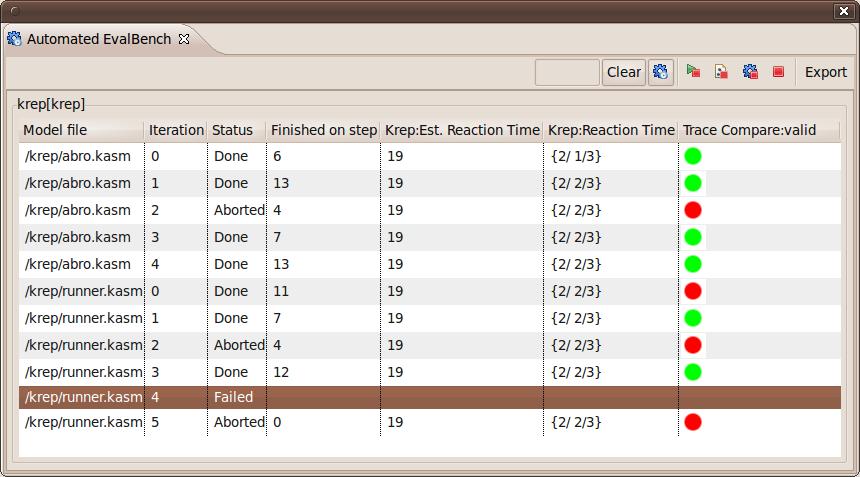
\includegraphics[scale=.45]{AutoView.png}
  \caption[Automation View showing the result of an automated execution.]%
  {Automation View showing the result of an automated execution.\protect}
  \label{fig:AutoView}
\end{figure}
The Automation View seen in Figure \ref{fig:AutoView} is used to display the results of an automated execution is a structured
way.

However it would be very undesirable if the user had to wait for the entire automated run
to finish before viewing any information. Therefore the view displays all information
that is currently available. 

The information is gathered from the output of the Automated Producers and also
includes status information produced by the automation itself. The first four
columns contain this status information:
\begin{enumerate}
 \item The first column shows the name of the model file that was simulated. This
might be the same for multiple subsequent rows as a model file might be simulated
with more than one iteration.
 \item The next column shows the index of the iteration that produced the given result.
 \item The third column displays the status that the execution that produced the result
is currently in:
\begin{itemize}
 \item \textbf{Created} : The current iteration has been created and is preparing to execute.
It is for example waiting for trace files to be opened or preliminary calculations.
 \item \textbf{Running} : The iteration is execution in the Execution Manager and performing
the desired number of steps.
 \item \textbf{Done} : The iteration completed successfully.
 \item \textbf{Aborted} : The iteration was aborted by the user or another component.
 \item \textbf{Failed} : The iteration failed to complete because of an error.
\end{itemize}
 \item The last column contains the step that the execution finished on.
\end{enumerate}
The following columns contain the information gathered from the Automated Producers.
In order to make the information easier to understand the column header not only displays
the name of the attribute but also the name of the component that produced the given
value.

If more than one execution file is simulated a new table will be created below the previous
tables. This is necessary because another execution file might contain different
components which produce different lists of results. These results would not fit into
the table of the previous executions. Another possibility would be to add additional columns
to the existing table. However this could increase the width of the table too much for the
user to still effectively read. Furthermore if the two execution files don't share any
components a shared table would look more confusing than helpful.

\subsection{Tool bar}
\label{section:AutoToolbar}
\begin{figure}
  \centering
  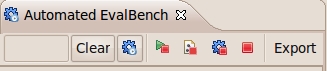
\includegraphics[scale=.8]{AutoToolbar.png}
  \caption[The tool bar in the automation view.]%
  {The tool bar in the automation view.\protect}
  \label{fig:AutoToolbar}
\end{figure}
The tool bar on the Automation View contains several actions for controlling the automated 
execution before, during and after its run (see Figure \ref{fig:AutoToolbar}).
The different controls have the following functionality (left-to-right):
\begin{enumerate}
 \item \textbf{Current Step Field} : During the automated run this field displays the
currently executing step. It is basically the same control as on the tool bar of the 
Execution Manager itself. The control was duplicated in this place in order to avoid
having to switch between the two views. This means that information about the currently
running execution is displayed in the Automation View.
 \item \textbf{Clear} : When the user initiates multiple automated runs after one another
the results are all displayed in the same view. This is the intended behavior as it should 
give the user the ability to compare automated runs with different inputs. However if the 
view gets filled with too many results the user needs an easy way to clear the view which
is realized through this button.
 \item \textbf{Automation Wizard} : The next button is used in order to launch the 
Automation Wizard. The button exists both here and on the Execution Manager's tool bar
in order to allow easy access to the automation.
 \item The next four buttons are used for performing one of the skipping actions supported
by the Cancel Manager (see Section \ref{section:CancelManager}):
\begin{enumerate}
 \item \textbf{Skip iteration} : This button allows the user to perform a 
deferred termination of the current iteration and proceed to the next index.
 \item \textbf{Skip model file} : This button has the same functionality as the one described
above but it will also skip to the next model file after aborting the current iteration. 
 \item \textbf{Skip execution file} : This button is used to skip an entire execution file.
 \item \textbf{Cancel automated execution} : The last button in this group is used to initiate a deferred
termination of the entire execution. This has the same functionality as pressing ``Cancel'' inside the 
progress monitor dialog.
\end{enumerate}
 \item \textbf{Export} : The export button is used for opening a dialog to export the currently displayed
results to an external format. This feature is explained in Section \ref{section:AutoExportResults}.
\end{enumerate}

\subsection{Exporting Results}
\label{section:AutoExportResults}
As described in Section \ref{section:AutoView} a number of tables is used to display the results in the view.
However these tables are not persistent i.e. they are removed when the program is closed.
In order to keep the results for analysis a method had to be found to export them into
an external format.

The button on the tool bar first opens a dialog that shows all available types that the results can
be exported to. The next window prompts the user to enter file names for the exported files.
Since the exported files are supposed to be used in other applications as well the standard 
\ac{OS} file chooser is used instead of the workspace file chooser.

\listingjava
\showlistingex{code/CSVExample.txt}
{Java}
{Example of a table exported to CSV.}
{list:CSVExample}
{t}
% generated by KIEM
% required packages:
% \usepackage{multicol}
% \usepackage{multirow}
\begin{table}[b]
\begin{tabular}{| l | p{1.2cm} | p{1.2cm} | p{1.2cm} | p{1cm} | p{1.4cm} | p{0.5cm} | } \hline
\multicolumn{4}{|c|}{}
 & \multicolumn{2}{c|}{Krep}
 & \multicolumn{1}{c|}{Trace Compare}
\\ \hline
Model file & Iteration & Status & Finished on step & Est. Reaction Time & Reaction Time & valid \\ \hline
\multirow{4}{*}{/krep/abro.kasm} & 1 & Done & 13 & 19 & {2/ 2/3} & true \\ 
 & 2 & Aborted & 4 & 19 & {2/ 2/3} & false \\ 
 & 3 & Done & 7 & 19 & {2/ 2/3} & true \\ 
 & 4 & Done & 13 & 19 & {2/ 2/3} & true \\ 
\hline
\multirow{6}{*}{/krep/runner.kasm} & 0 & Done & 11 & 19 & {2/ 2/3} & false \\ 
 & 1 & Done & 7 & 19 & {2/ 2/3} & true \\ 
 & 2 & Aborted & 4 & 19 & {2/ 2/3} & false \\ 
 & 3 & Done & 12 & 19 & {2/ 2/3} & true \\ 
 & 4 & Failed &  &  &  &  \\ 
 & 5 & Aborted & 0 & 19 & {2/ 2/3} & false \\ 
\hline
\end{tabular}
  \caption[Example of a table exported to \LaTeX .]%
  {Example of a table exported to \LaTeX .\protect}
\label{table:LatexExample}
\end{table}
To illustrate the results of such a transformation the table shown in Figure \ref{fig:AutoView} is
transformed in both formats. The resulting \ac{CSV} file can be seen in Listing \ref{list:CSVExample}. The same
results exported to \LaTeX can be viewed in Table \ref{table:LatexExample}.